\subsection{Problem 1: Regression Analysis of Insured Persons}
\subsubsection{Problem Description}
The objective of this problem is to analyze historical data concerning the number of insured persons over a ten-year period (1987–1996) and fit an appropriate regression model. \\
The goal is to analyze the dataset for potential outliers, evaluate linear, quadratic, and cubic polynomial fits to determine the most suitable model, and ultimately predict the number of insured persons for the year 1997. 

\subsubsection{Hand Analysis}
We will first analyze the \textbf{original dataset}, then remove the outlier and refit.

\paragraph{Step 1: Transform Year for Numerical Stability} \mbox{} \\
The dataset provides the yearly count of insured persons ($y$), which is modeled against the number of years since 1987 ($x = \text{Year} - 1987$, such that $x \in \{0, 1, \dots, 9\}$). 

\begin{table}[H]
\centering
\begin{tabular}{|c|cccccccccc|}
\hline
$x$ & 0 & 1 & 2 & 3 & 4 & 5 & 6 & 7 & 8 & 9 \\
\hline
$y$ & 12400 & 10900 & 10000 & 1050 & 9500 & 8900 & 8000 & 7800 & 7600 & 7200 \\
\hline
\end{tabular}
\end{table}

\paragraph{Step 2: Fit Models (Original Data)} \mbox{} \\
We consider the following polynomial models:
\begin{align*}
\text{Linear:} \quad & y = a_0 + a_1 x \\
\text{Quadratic:} \quad & y = b_0 + b_1 x + b_2 x^2 \\
\text{Cubic:} \quad & y = c_0 + c_1 x + c_2 x^2 + c_3 x^3
\end{align*}

\subparagraph{Linear Regression Analysis} \mbox{} \\
For the original dataset with $n=10$ points, we perform a detailed linear regression analysis to fit the model $y = a_0 + a_1x$.
\textbf{Computing the Regression Coefficients:}

\begin{table}[H]
\centering
\begin{tabular}{|c|c|c|c|c|c|c|c|}
\hline
$x_i$ & $y_i$ & $(x_i - \bar{x})$ & $(y_i - \bar{y})$ & $(x_i - \bar{x})^2$ & $(y_i - \bar{y})^2$ & $(x_i - \bar{x})(y_i - \bar{y})$ \\
\hline
0 & 12400 & $-4.5$ & 4065 & 20.25 & 16524225 & $-18292.5$ \\
1 & 10900 & $-3.5$ & 2565 & 12.25 & 6579225 & $-8977.5$ \\
2 & 10000 & $-2.5$ & 1665 & 6.25 & 2772225 & $-4162.5$ \\
3 & 1050 & $-1.5$ & $-7285$ & 2.25 & 53070225 & $10927.5$ \\
4 & 9500 & $-0.5$ & 1165 & 0.25 & 1357225 & $-582.5$ \\
5 & 8900 & $0.5$ & 565 & 0.25 & 319225 & $282.5$ \\
6 & 8000 & $1.5$ & $-335$ & 2.25 & 112225 & $-502.5$ \\
7 & 7800 & $2.5$ & $-535$ & 6.25 & 286225 & $-1337.5$ \\
8 & 7600 & $3.5$ & $-735$ & 12.25 & 540225 & $-2572.5$ \\
9 & 7200 & $4.5$ & $-1135$ & 20.25 & 1288225 & $-5107.5$ \\
\hline
\multicolumn{2}{|c|}{\textbf{Sum}} & & & 82.5 & $8.29 \times 10^7$ & $-30325$ \\
\hline
\end{tabular}
\end{table}
\begin{itemize}
    \item \textbf{Mean:} $\bar{x} = \frac{0+1+2+\cdots+9}{10} = 4.5$
    \item \textbf{Mean:} $\bar{y} = \frac{\sum y_i}{10} = 8335$
\end{itemize}
Using the regression formulas:
\[
a_1 = \frac{\sum (x_i - \bar{x})(y_i - \bar{y})}{\sum (x_i - \bar{x})^2} = \frac{-30325}{82.5} \approx -367.58
\]

\[
a_0 = \bar{y} - a_1\bar{x} = 8335 - (-367.58)(4.5) = 8335 + 1654.09 \approx 9989.09
\]

Thus, the linear model for the original data is:
\[
y \approx 9989.1 - 367.6x
\]

\textbf{Steps for Computing $SSE$ and $R^2$:}
\begin{enumerate}
    \item Compute predicted values for each point using the fitted model:
    \[
    \hat{y}_i = a_0 + a_1x_i
    \]
    \item Compute residuals (prediction errors):
    \[
    e_i = y_i - \hat{y}_i
    \]
    \item Square and sum the residuals to obtain the error sum of squares:
    \[
    SSE = \sum e_i^2 = \sum (y_i - \hat{y}_i)^2
    \]
    \item Compute the total variability around the mean:
    \[
    SST = \sum (y_i - \bar{y})^2
    \]
    \item Compute the coefficient of determination:
    \[
    R^2 = 1 - \frac{SSE}{SST}
    \]
\end{enumerate}

Substituting the values for the original dataset:
\[
SSE_{\text{lin}} = \sum (y_i - \hat{y}_i)^2 \approx 7.17 \times 10^7
\]

\[
R^2_{\text{lin}} = 1 - \frac{SSE_{\text{lin}}}{SST} \approx 1 - \frac{7.17 \times 10^7}{8.29 \times 10^7} \approx 0.135
\]

\textbf{Observation:} The linear model yields a low $R^2 \approx 0.135$, indicating a poor fit. The outlier at $(x=3, y=1050)$ severely distorts the linear trend.

\subparagraph{Quadratic Model} \mbox{} \\
A quadratic model takes the form $y = b_0 + b_1 x + b_2 x^2$. 

Using the matrix method, define
\[
X = \begin{bmatrix}
1 & x_1 & x_1^2 \\
\vdots & \vdots & \vdots \\
1 & x_n & x_n^2
\end{bmatrix},
\quad
\beta = \begin{bmatrix} b_0 \\ b_1 \\ b_2 \end{bmatrix},
\quad
y = \begin{bmatrix} y_1 \\ \vdots \\ y_n \end{bmatrix}
\]
and solve the normal equations
\[
(X^T X)\beta = X^T y.
\]

For the original data ($n=10$, $x=0,\dots,9$):
\[
X^T X =
\begin{bmatrix}
10 & 45 & 285 \\
45 & 285 & 2025 \\
285 & 2025 & 15333
\end{bmatrix},
\quad
X^T y =
\begin{bmatrix}
83350 \\
344750 \\
2174650
\end{bmatrix}.
\]

Solving gives
\[
\beta =
\begin{bmatrix}
11627.73 \\
-1596.55 \\
136.55
\end{bmatrix},
\]
so the fitted quadratic model is
\[
\hat{y} = 11627.73 - 1596.55x + 136.55x^2.
\]

This model can bend around the outlier more than a line, and its fit metrics are:

\[
SSE_{\text{quad}} \approx 6.19 \times 10^7
\]

\[
R^2_{\text{quad}} \approx 1 - \frac{6.19 \times 10^7}{8.29 \times 10^7} \approx 0.253
\]

\textbf{Observation:} The quadratic model shows improvement over the linear model ($R^2$ increases from $0.135$ to $0.253$), but still provides a weak overall fit. The outlier prevents the quadratic from capturing the underlying trend across all points.

\subparagraph{Cubic Model} \mbox{} \\
A cubic model takes the form $y = c_0 + c_1 x + c_2 x^2 + c_3 x^3$.

Using the matrix method, define
\[
X = \begin{bmatrix}
1 & x_1 & x_1^2 & x_1^3 \\
\vdots & \vdots & \vdots & \vdots \\
1 & x_n & x_n^2 & x_n^3
\end{bmatrix},
\quad
\beta = \begin{bmatrix} c_0 \\ c_1 \\ c_2 \\ c_3 \end{bmatrix},
\]
and solve
\[
(X^T X)\beta = X^T y.
\]

For the original data:
\[
X^T X =
\begin{bmatrix}
10 & 45 & 285 & 2025 \\
45 & 285 & 2025 & 15333 \\
285 & 2025 & 15333 & 120825 \\
2025 & 15333 & 120825 & 978405
\end{bmatrix},
\quad
X^T y =
\begin{bmatrix}
83350 \\
344750 \\
2174650 \\
15383150
\end{bmatrix}.
\]

Solving gives
\[
\beta =
\begin{bmatrix}
13113.15 \\
-4313.93 \\
932.31 \\
-58.95
\end{bmatrix},
\]
so the fitted cubic model is
\[
\hat{y} = 13113.15 - 4313.93x + 932.31x^2 - 58.95x^3.
\]

With 4 parameters for 10 data points, the cubic model has more flexibility to bend around the outlier. Its fit metrics are:

\[
SSE_{\text{cubic}} \approx 5.11 \times 10^7
\]

\[
R^2_{\text{cubic}} \approx 1 - \frac{5.11 \times 10^7}{8.29 \times 10^7} \approx 0.383
\]

\textbf{Observation:} The cubic model exhibits the highest $R^2 \approx 0.383$, but this improvement is still largely driven by the model's increased flexibility to fit the extreme outlier rather than capturing a genuine cubic underlying trend.

\subparagraph{Conclusion for Original Data} \mbox{} \\
Although the cubic model has the highest $R^2$ value among the three models fitted to the original data, the overall poor performance across all models (even the best $R^2 \approx 0.383$ explains only about 38\% of variance) demonstrates the severe impact of the outlier. The outlier at $(x=3, y=1050)$ fundamentally distorts the regression analysis, and no simple polynomial model can adequately fit both this extreme point and the general declining trend in the remaining data. This observation motivates the need for outlier detection and removal before proceeding with final model selection.

\paragraph{Step 3: Remove Outlier} \mbox{} \\
Removing the obvious outlier $(x=3, y=1050)$ leaves $n=9$ valid points.

\paragraph{Step 4: Fit Models Without Outlier} \mbox{} \\
\subparagraph{Linear Regression Analysis} \mbox{} \\
For the remaining $n = 9$ data points, the $x$ values are $\{0, 1, 2, 4, 5, 6, 7, 8, 9\}$. The detailed computations are shown below:

\begin{table}[H]
\centering
\begin{tabular}{|c|c|c|c|c|c|c|}
\hline
$x_i$ & $y_i$ & $(x_i - \bar{x})$ & $(y_i - \bar{y})$ & $(x_i - \bar{x})^2$ & $(y_i - \bar{y})^2$ & $(x_i - \bar{x})(y_i - \bar{y})$ \\
\hline
0 & 12400 & $-4.667$ & 3255.556 & 21.778 & 10598641.98 & $-15192.59$ \\
1 & 10900 & $-3.667$ & 1755.556 & 13.444 & 3082716.05 & $-6437.04$ \\
2 & 10000 & $-2.667$ & 855.556 & 7.111 & 731975.31 & $-2281.48$ \\
4 & 9500 & $-0.667$ & 355.556 & 0.444 & 126419.75 & $-237.04$ \\
5 & 8900 & $0.333$ & $-244.444$ & 0.111 & 59753.09 & $-81.48$ \\
6 & 8000 & $1.333$ & $-1144.444$ & 1.778 & 1309753.09 & $-1525.93$ \\
7 & 7800 & $2.333$ & $-1344.444$ & 5.444 & 1807530.86 & $-3137.04$ \\
8 & 7600 & $3.333$ & $-1544.444$ & 11.111 & 2385308.64 & $-5148.15$ \\
9 & 7200 & $4.333$ & $-1944.444$ & 18.778 & 3780864.20 & $-8425.93$ \\
\hline
\multicolumn{2}{|c|}{\textbf{Sum}} & & & 80.000 & $2.39 \times 10^7$ & $-42466.67$ \\
\hline
\end{tabular}
\end{table}
\begin{itemize}
    \item \textbf{Mean:} $\bar{x} = \frac{0+1+2+4+\cdots+9}{9} = 4.667$
    \item \textbf{Mean:} $\bar{y} = \frac{\sum y_i}{9} = 9144.44$
\end{itemize}

Using the regression formulas:
\[
a_1 = \frac{\sum (x_i - \bar{x})(y_i - \bar{y})}{\sum (x_i - \bar{x})^2} = \frac{-42466.67}{80} \approx -530.83
\]

\[
a_0 = \bar{y} - a_1\bar{x} = 9144.44 - (-530.83)(4.667) = 9144.44 + 2477.23 \approx 11621.67
\]

Thus, the best-fit linear equation is:
\[
    y \approx 11621.67 - 530.83x
\]

Substituting the cleaned-data values into the previously defined $SSE$ and $R^2$ equations:
\begin{align*}
    SSE_{\text{lin}} &= \sum (y_i - \hat{y}_i)^2 \approx 1.34 \times 10^6 \\
    R^2_{\text{lin}} &= 1 - \frac{SSE_{\text{lin}}}{SST} \approx 1 - \frac{1.34 \times 10^6}{2.39 \times 10^7} \approx 0.944
\end{align*}

The linear model already provides an excellent fit with $R^2 \approx 0.944$.

\subparagraph{Quadratic Model} \mbox{} \\
A quadratic model takes the form $y = b_0 + b_1 x + b_2 x^2$.

Using the matrix method defined previously, for the cleaned data:
\[
X^T X =
\begin{bmatrix}
9 & 42 & 276 \\
42 & 276 & 1998 \\
276 & 1998 & 15252
\end{bmatrix},
\quad
X^T y =
\begin{bmatrix}
82300 \\
341600 \\
2165200
\end{bmatrix}.
\]

Solving gives
\[
\beta =
\begin{bmatrix}
12024.17 \\
-863.13 \\
37.44
\end{bmatrix},
\]
so the fitted quadratic model is
\[
\hat{y} = 12024.17 - 863.13x + 37.44x^2.
\]

Its fit metrics are:
\[
SSE_{\text{quad}} \approx 6.57 \times 10^5
\]
\[
R^2_{\text{quad}} \approx 1 - \frac{6.57 \times 10^5}{2.39 \times 10^7} \approx 0.972
\]

\textbf{Observation:} The quadratic model improves the fit over linear ($R^2$ increases from $0.944$ to $0.972$), but adds one extra parameter.

\subparagraph{Cubic Model} \mbox{} \\
A cubic model takes the form $y = c_0 + c_1 x + c_2 x^2 + c_3 x^3$.

Using the matrix method defined previously, for the cleaned data:

For the cleaned data:
\[
X^T X =
\begin{bmatrix}
9 & 42 & 276 & 1998 \\
42 & 276 & 1998 & 15252 \\
276 & 1998 & 15252 & 120582 \\
1998 & 15252 & 120582 & 977676
\end{bmatrix},
\quad
X^T y =
\begin{bmatrix}
82300 \\
341600 \\
2165200 \\
15354800
\end{bmatrix}.
\]

Solving gives
\[
\beta =
\begin{bmatrix}
12204.42 \\
-1221.74 \\
140.17 \\
-7.46
\end{bmatrix},
\]
so the fitted cubic model is
\[
\hat{y} = 12204.42 - 1221.74x + 140.17x^2 - 7.46x^3.
\]

Its fit metrics are:
\[
SSE_{\text{cubic}} \approx 5.09 \times 10^5
\]
\[
R^2_{\text{cubic}} \approx 1 - \frac{5.09 \times 10^5}{2.39 \times 10^7} \approx 0.979
\]

\textbf{Observation:} The cubic model gives the highest $R^2$, but the improvement from quadratic ($0.972 \to 0.979$) is modest relative to the extra complexity.

\subparagraph{Conclusion for Cleaned Data} \mbox{} \\
All three models fit the cleaned dataset well. However, following the same model-selection principle used in Step 2 (favor simpler models unless improvement is substantial), the linear model remains the preferred choice for interpretation and forecasting. Although quadratic and cubic models increase $R^2$, the linear trend already captures the dominant behavior after outlier removal and avoids unnecessary model complexity.

\paragraph{Step 5: Predict for 1997} \mbox{} \\
The year 1997 corresponds to $x=10$ (since $x=\text{Year}-1987$).
Using the linear model $y = 11621.67 - 530.83x$:
\[
y_{1997} = 11621.67 - 530.83(10) = 11621.67 - 5308.30 = 6313.37
\]

Thus, the predicted number of insured persons in 1997 is approximately $\boxed{6313}$.

\subsubsection{Simulation Analysis}

\paragraph{(a) Model Fitting and $R^2$ Comparison} \mbox{} \\
A scatterplot of the original data shows a generally decreasing trend with a sharp drop at $x=3$. We fit linear, quadratic, and cubic models and compute $R^2$:

\begin{figure}[H]
    \centering
    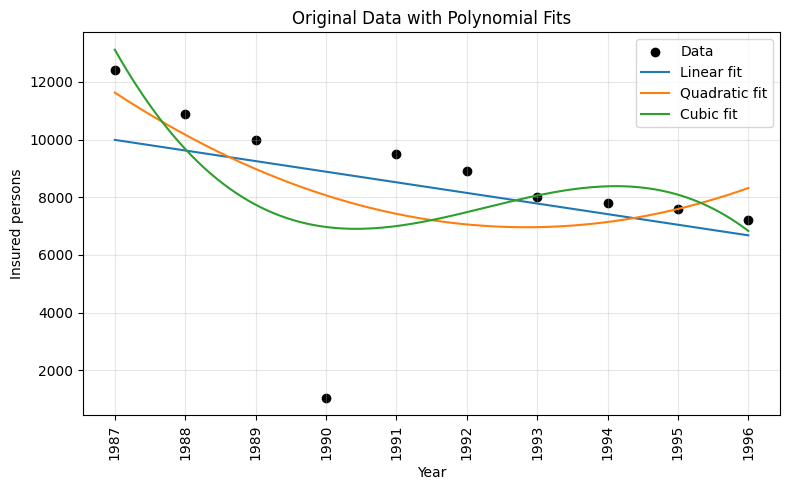
\includegraphics[width=0.6\textwidth]{figures/Original Data with Polynomial Fits.png}
    \caption{Scatterplot of insured persons vs. years since 1987 with polynomial fits (original data)}
    \label{fig:scatter}
\end{figure}

\begin{figure}[H]
    \centering
    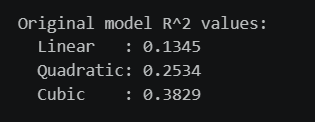
\includegraphics[height=0.15\textwidth]{figures/Original R-Squared.png}
    \caption{R-squared values for the original data}
    \label{fig:originalr2}
\end{figure}

\textbf{Observation:} All models yield relatively low $R^2$ values. Even the cubic model explains less than $40\%$ of the variance, indicating a poor overall fit due to the outlier.

\textbf{Conclusion:} Although the cubic model has the highest $R^2$, the improvement is artificially limited and does not adequately capture the generalized data behavior.

\paragraph{(b) Outlier Removal and Re-fitting} \mbox{} \\
From the initial scatterplot, the point $(x=3, y=1050)$ is clearly outside the general trend and rightfully treated as an outlier. After removing this point, the data demonstrates a strong linear decreasing pattern.

\begin{figure}[H]
    \centering
    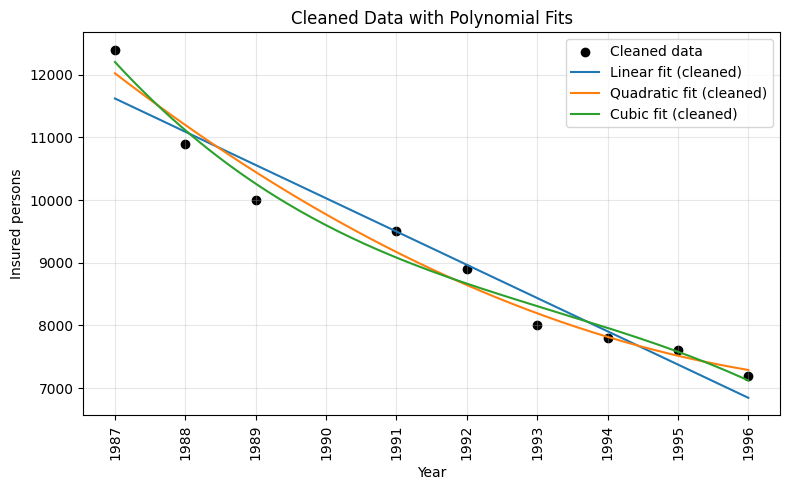
\includegraphics[width=0.6\textwidth]{figures/Cleaned Data with Polynomial Fits.png}
    \caption{Scatterplot of insured persons vs. years since 1987 with polynomial fits (cleaned data)}
    \label{fig:scatter2}
\end{figure}

Recomputing the models yields the following metrics:

\begin{figure}[H]
    \centering
    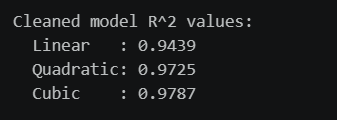
\includegraphics[height=0.15\textwidth]{figures/Cleaned R-Squared.png}
    \caption{R-squared values for cleaned data}
    \label{fig:cleanr2}
\end{figure}

\textbf{Conclusion:} The linear model already provides an excellent fit. Higher-order models offer only marginal mathematical improvement and introduce unnecessary complexity.
\[
\boxed{\text{Best model: Linear}}
\]

\paragraph{(c) Graphical Representation} \mbox{} \\
The scatterplot for the cleaned data is plotted along with the best-fit linear function:
\[
y \approx 11621.67 - 530.83x
\]
The fitted line closely follows the data trend after outlier removal, visually validating our model choice.

\paragraph{(d) Prediction for 1997} \mbox{} \\
For the year 1997 ($x = 10$):

\begin{figure}[H]
    \centering
    
\includegraphics[width=0.6\textwidth]{figures/Prediction.png}
    \caption{Best cleaned model providing a forecast for 1997}
    \label{fig:p1_prediction_1997}
\end{figure}

Using the best-fit linear model:
\[
y = 11621.67 - 530.83(10) = 6313.37
\]
\[
\boxed{y_{1997} \approx 6313}
\]

\paragraph{Final Interpretation} \mbox{} \\
The presence of the single outlier significantly degraded the initial model performance. After removing it, the dataset is very well-described by a simpler linear model, which ultimately provides a more reliable and robust prediction for future values.